% ------------------------------------------------------------%
% Relatório de Química - Prática: Teor de etanol na gasolina
% Template IFSC (ifscarticle) - Câmpus São José
% Compilar: latexmk -pdf relatorio_corrigido.tex
% ------------------------------------------------------------%
\documentclass[11pt]{ifscarticle}
\usepackage{ifscutils}
\usepackage[alf]{abntex2cite}
\usepackage{setspace}
\usepackage{indentfirst}

\AtBeginDocument{\thispagestyle{empty}}

\begin{document}

% ------------------------------------------------------------%
% Capa
% ------------------------------------------------------------%
\begin{titlepage}
\begin{center}

\includegraphics[scale=.7]{./figuras/ifsc-v}
\vspace{2.5cm}

\rule{\linewidth}{0.5pt}\\[6pt]
\doublespacing
{\huge\bfseries Determinação do Teor de Etanol na Gasolina}\\[4pt]
{\large Relatório da prática de laboratório}\\

\rule{\linewidth}{2pt}\\[10pt]
\vspace{1cm}
\end{center}

\begin{minipage}{.9\linewidth}
\begin{minipage}{0.20\textwidth}
\begin{flushleft}\large
\textbf{Curso:}\\
\textbf{Componente:}\\
\textbf{Professor:}\\
\end{flushleft}
\end{minipage}
\hfill
\begin{minipage}{0.78\textwidth}
\begin{flushleft}\large
Engenharia de Telecomunicações\\
Química\\
Maick Meneguzzo Prado\\
\end{flushleft}
\end{minipage}
\end{minipage}

\vspace{2.5cm}

\begin{minipage}{.9\linewidth}
\begin{flushright}
\textbf{Alunos:}\\
Victor Evandro de Lima Guerra\\
Diogo Ramos Santarosa\\
\end{flushright}
\end{minipage}

\vfill

\begin{center}
São José, 12 de agosto de 2026
\end{center}
\end{titlepage}

% ------------------------------------------------------------%
% Sumário
% ------------------------------------------------------------%
\tableofcontents
\clearpage
\onehalfspacing

% ------------------------------------------------------------%
% Início do documento
% ------------------------------------------------------------%
\section{Introdução}

O petróleo é uma mistura complexa formada principalmente por hidrocarbonetos, além de pequenas quantidades de compostos contendo enxofre, nitrogênio, oxigênio e metais. Na forma bruta, ele possui aplicação direta limitada e, por isso, precisa passar por diferentes etapas de processamento em uma refinaria. Uma das principais operações é a destilação fracionada, na qual os componentes são separados de acordo com suas diferentes faixas de temperatura de ebulição. Desse processo são obtidas frações como gás liquefeito de petróleo, nafta, querosene, óleo diesel, óleos lubrificantes e frações mais pesadas utilizadas na produção de asfalto \cite{thomas2004}. Entre os produtos derivados do petróleo, a gasolina possui grande importância econômica devido ao seu uso como combustível em veículos com motores do ciclo Otto.

A gasolina comercial não é formada por uma única substância, mas por uma mistura de diferentes hidrocarbonetos, principalmente compostos com cadeias contendo aproximadamente de cinco a doze átomos de carbono. Esses hidrocarbonetos apresentam baixa polaridade e, consequentemente, pouca afinidade com substâncias polares como a água \cite{solomons2012,atkins2012}. Essa diferença de polaridade explica por que gasolina e água formam duas fases distintas quando colocadas em contato. Tal comportamento é importante para esta prática experimental, pois permite utilizar a água como meio para retirar parte do etanol presente na gasolina e, a partir da variação de volume observada, realizar uma estimativa do teor desse álcool na amostra.

O desempenho da gasolina em um motor depende de diferentes propriedades, entre elas sua resistência à detonação. Essa característica é expressa pelo índice de octanagem, que indica a capacidade do combustível de suportar a compressão dentro do cilindro sem sofrer combustão prematura \cite{brown2016}. Quando a mistura ar-combustível entra em combustão antes do momento adequado, podem ocorrer perda de rendimento, aumento de ruído e esforços mecânicos indesejados no motor. Ao longo do desenvolvimento dos combustíveis automotivos, diferentes substâncias foram utilizadas para elevar a resistência da gasolina à detonação.

Durante parte do século XX, compostos à base de chumbo foram utilizados como agentes antidetonantes. Esses compostos eram eficientes, mas foram progressivamente abandonados devido aos impactos ambientais e aos efeitos tóxicos do chumbo sobre a saúde humana \cite{baird2011}. A substituição desses aditivos exigiu outras soluções para melhorar as propriedades da gasolina, e o etanol passou a desempenhar papel importante nesse contexto. Além de contribuir para a octanagem, o etanol contém oxigênio em sua estrutura molecular, o que também influencia o processo de combustão.

Quimicamente, o etanol apresenta uma característica particularmente importante para o experimento realizado. Sua molécula possui uma extremidade polar, associada ao grupo hidroxila (OH), e uma parte formada por cadeia carbônica, que apresenta caráter menos polar. Essa estrutura faz com que o etanol consiga interagir tanto com a gasolina quanto com a água. Quando a gasolina contendo etanol é colocada em contato com uma fase aquosa, ocorre uma redistribuição do álcool entre as duas fases, com transferência preferencial para a água, favorecida pelas interações intermoleculares estabelecidas entre as moléculas de etanol e de água \cite{atkins2012,solomons2012}. É justamente essa propriedade que torna possível a determinação aproximada do teor de etanol por meio de um ensaio simples de extração.

No Brasil, o etanol anidro é adicionado obrigatoriamente à gasolina C comercializada nos postos de combustíveis. O percentual dessa mistura é definido por regulamentação e pode ser alterado conforme decisões de política energética e especificações técnicas. Em 2025, o Conselho Nacional de Política Energética elevou o percentual obrigatório de etanol anidro de 27\% para 30\%, estabelecendo a mistura conhecida como E30 \cite{cnpe9,mme_e30}. Em 2026, foi aprovada temporariamente uma nova elevação para 32\% \cite{cnpe2026}. Essas mudanças estão relacionadas à Política Combustível do Futuro \cite{leicombfuturo}.

A quantidade de etanol presente na gasolina também é relevante do ponto de vista do controle de qualidade. Um teor diferente daquele estabelecido para determinada especificação pode alterar propriedades do combustível e afetar seu desempenho. Existem procedimentos padronizados para a determinação do teor de etanol, entre eles o método descrito na ABNT NBR 13992 \cite{nbr13992}. Esse método utiliza condições de ensaio padronizadas e solução aquosa apropriada para favorecer a separação entre as fases e permitir uma determinação mais confiável.

Na prática realizada em laboratório, porém, foi empregado um procedimento didático simplificado, utilizando água pura, proveta graduada e leitura direta da variação de volume da fase aquosa. Os resultados obtidos são, portanto, estimativas experimentais e não uma análise oficial de conformidade. O procedimento ainda permite visualizar com clareza conceitos importantes de química, como polaridade, solubilidade, interações intermoleculares, separação de fases e influência da composição química nas propriedades de um combustível.

O objetivo deste trabalho foi estimar o teor de etanol presente em duas amostras de gasolina por meio da extração com água, comparar os resultados obtidos pelos diferentes grupos da turma e relacionar o comportamento observado às propriedades químicas das substâncias envolvidas. Buscou-se também discutir as limitações do método utilizado e comparar, de maneira apenas indicativa, os valores experimentais com os percentuais de etanol adotados para a gasolina comercial.

\section{Metodologia}

Foram analisadas duas amostras de gasolina. A primeira havia sido levada ao laboratório no dia da prática, sendo identificada neste relatório como Posto A. A segunda já se encontrava no laboratório e não possuía informação sobre o posto de origem nem sobre a data de coleta; ela foi identificada como Posto B.

Para cada amostra, foram medidos \SI{50}{\milli\liter} de gasolina em uma proveta de \SI{100}{\milli\liter}. Em seguida, adicionaram-se \SI{50}{\milli\liter} de água. A proveta foi agitada cuidadosamente e mantida em repouso por alguns minutos, até que a separação entre as fases pudesse ser observada.

Após o repouso, formaram-se duas fases. A fase inferior, predominantemente aquosa, apresentou volume superior aos \SI{50}{\milli\liter} adicionados inicialmente. Esse aumento foi atribuído à transferência de etanol da gasolina para a água. A fase superior correspondeu principalmente à gasolina.

O roteiro da prática utilizou o cálculo simplificado

\begin{equation}
\%\,\text{etanol} =
\frac{V_{\text{extraído}}}{V_{\text{gasolina}}}\times 100,
\end{equation}

em que $V_{\text{extraído}}$ corresponde ao aumento de volume observado na fase aquosa e $V_{\text{gasolina}}$ é o volume inicial de gasolina, igual a \SI{50}{\milli\liter}.

Esse procedimento não deve ser confundido com o ensaio normalizado para fins de controle de qualidade. O método padronizado emprega solução aquosa salina, condições de ensaio definidas e tratamento específico para o cálculo do teor de etanol \cite{nbr13992}. Os resultados apresentados neste relatório foram mantidos de acordo com o roteiro experimental utilizado em aula e não representam uma determinação oficial de conformidade.

A turma foi dividida em três grupos, e cada grupo realizou o procedimento com as duas amostras. A partir das três leituras, foram calculadas a média e o desvio padrão amostral,

\begin{equation}
s =
\sqrt{
\frac{\sum_{i=1}^{n}(x_i-\bar{x})^2}{n-1}
},
\end{equation}

em que $x_i$ representa cada resultado, $\bar{x}$ a média e $n=3$ o número de repetições.

\section{Resultados e Discussão}

A separação entre as fases foi observada nas duas amostras, conforme apresentado na Figura~\ref{fig:provetas}. A fase inferior ficou visualmente mais clara e aumentou de volume após o contato com a gasolina, enquanto a fase superior manteve a coloração característica do combustível.

\begin{figure}[htb]
    \centering
    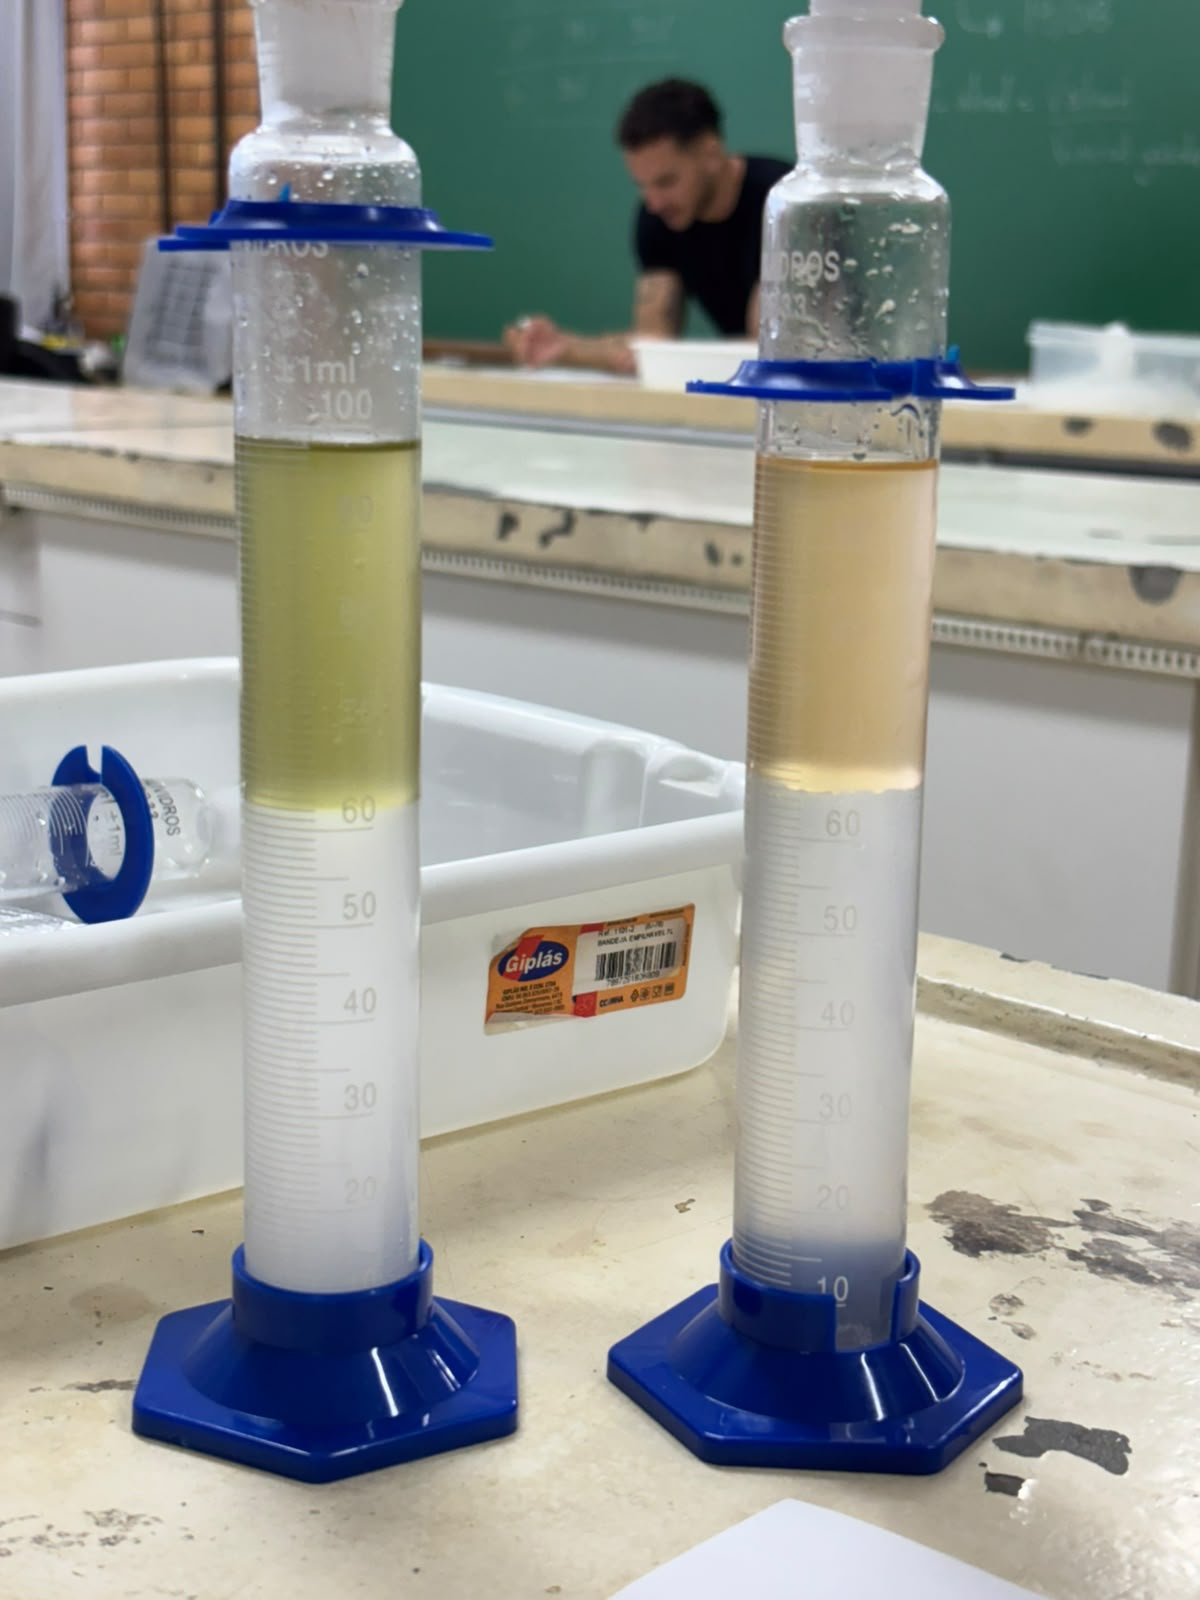
\includegraphics[width=0.5\textwidth]{figura_provetas.jpeg}
    \caption{Provetas após a adição de água e o período de repouso, com formação de uma fase aquosa inferior e uma fase orgânica superior.}
    \label{fig:provetas}
    \par\smallskip
    {\footnotesize Fonte: Autores (2026).}
\end{figure}

Esse comportamento pode ser explicado pela diferença de polaridade entre os componentes. Os hidrocarbonetos presentes na gasolina apresentam baixa afinidade com a água, enquanto o etanol possui um grupo hidroxila capaz de estabelecer interações favoráveis com moléculas de água. Ao entrar em contato com a fase aquosa, parte do etanol presente na gasolina é transferida para essa fase \cite{atkins2012,solomons2012}.

No grupo III, a amostra do Posto B apresentou aumento de \SI{13}{\milli\liter} na fase aquosa. Pelo cálculo utilizado na prática,

\begin{equation}
\%\,\text{etanol} =
\frac{13}{50}\times 100 = 26\%.
\end{equation}

Para a amostra do Posto A, o aumento observado foi de \SI{15}{\milli\liter}, resultando em

\begin{equation}
\%\,\text{etanol} =
\frac{15}{50}\times 100 = 30\%.
\end{equation}

Os resultados dos três grupos são apresentados na Tabela~\ref{tab:resultados}.

\begin{table}[htb]
    \centering
    \caption{Teor de etanol estimado pelos três grupos para as duas amostras de gasolina.}
    \label{tab:resultados}
    \begin{tabular}{ccc}
        \toprule
        Grupo & Posto A & Posto B \\
        \midrule
        I   & 30\% & 28\% \\
        II  & 34\% & 30\% \\
        III & 30\% & 26\% \\
        \midrule
        Média          & 31,3\% & 28,0\% \\
        Desvio padrão  & 2,3 p.p. & 2,0 p.p. \\
        \bottomrule
    \end{tabular}
    \par\smallskip
    {\footnotesize Fonte: Autores (2026).}
\end{table}

A amostra do Posto A apresentou valores maiores que a amostra do Posto B nas três repetições. As médias foram de 31,3\% e 28,0\%, respectivamente. Os desvios padrão, de 2,3 e 2,0 pontos percentuais, mostram que houve variação entre as leituras dos grupos, o que é esperado em um procedimento baseado na leitura visual da interface entre duas fases. Como o cálculo empregado parte sempre de um volume fixo de \SI{50}{\milli\liter} de gasolina, cada mililitro lido na fase aquosa corresponde a exatamente 2 pontos percentuais de etanol. Dividindo os desvios por esse fator, obtém-se \SI{1,15}{\milli\liter} e \SI{1,00}{\milli\liter} de variação na leitura da proveta, valores da mesma ordem da menor divisão da escala utilizada. Isso indica que a dispersão observada está associada principalmente ao procedimento de leitura, e não a uma diferença real entre as provetas preparadas por cada grupo. Como foram realizadas apenas três repetições por amostra, os valores médios devem ser tratados como estimativas, sem que se extraia deles uma comparação quantitativa mais rigorosa.

Entre as principais fontes de incerteza estão a resolução da proveta, a definição visual da interface entre os líquidos, a leitura do menisco, a agitação da mistura e a ausência de controle de temperatura. A mistura entre água e etanol também não apresenta comportamento volumétrico perfeitamente aditivo, o que limita a interpretação direta da variação de volume \cite{atkins2012}.

Os valores podem ser comparados apenas de forma indicativa com os percentuais definidos para a gasolina C. A amostra do Posto A, coletada no período da prática, apresentou média próxima ao valor de 32\% aprovado pelo CNPE em 2026. Já a amostra do Posto B apresentou média menor, próxima de percentuais utilizados anteriormente. Como não há informação sobre a data de aquisição dessa segunda amostra, não é possível relacionar seu resultado a uma regulamentação específica.

Também não é adequado concluir, a partir deste ensaio didático, que uma das amostras esteja adulterada ou fora de especificação. Para esse tipo de conclusão seria necessário aplicar o procedimento padronizado, com os reagentes, condições e critérios de aceitação estabelecidos para controle de qualidade \cite{nbr13992}.

\section{Conclusão}

O experimento permitiu observar a separação entre a gasolina e a fase aquosa e estimar o teor de etanol presente em duas amostras. O resultado está de acordo com o comportamento esperado a partir da polaridade das substâncias: a gasolina permaneceu predominantemente na fase superior, enquanto o etanol apresentou maior afinidade pela fase aquosa.

As médias obtidas pelo procedimento adotado foram de 31,3\% para a amostra do Posto A e 28,0\% para a amostra do Posto B, com desvios padrão de 2,3 e 2,0 pontos percentuais, respectivamente. A diferença entre as médias foi observada de forma consistente nos três grupos, embora o número reduzido de repetições e as limitações da leitura em proveta não permitam uma interpretação quantitativa rigorosa.

A prática mostrou que o método de extração com água é útil para demonstrar o comportamento do etanol em uma mistura com gasolina, mas os resultados devem ser considerados apenas estimativas, já que o procedimento utilizado em aula não reproduz integralmente o método padronizado. Os valores obtidos não são suficientes, por si só, para afirmar conformidade ou adulteração das amostras.

% ------------------------------------------------------------%
% Referências
% ------------------------------------------------------------%
\clearpage
\bibliography{referencias}

\end{document}
